\section{Method}
This section is organized around three key questions in the context of ML license analysis: (i) How to determine the corresponding conditions in licenses for certain model reuse mechanisms? (ii) How to capture the dependency structure of a machine learning project? (iii) What types of non-compliance exist in ML projects and how to assess them?
We will present our solutions to these questions in the following sections.

\subsection{Taxonomy for ML License Analysis}
Determining the corresponding conditions in licenses is a challenging task for ML projects due to the conceptual ambiguities in existing licensing language and the disorganization in current ML licensing practices.
For example, CC-BY-ND prohibits the sharing of derivatives of licensed materials.
However, its definition of making derivatives is unclear in the context of ML domain.
For instance, should embeddings of a corpus be considered a derivative work upon that corpus?
Unfortunately, even though Creative Commons provides a flow chart to illustrate the trigger conditions of CC licenses in the context of AI activity~\cite{creative2023artificial}, it raises another question: \textit{Is the output considered protectable copyright subject matter?}
The answer depends on how the embedding activity is interpreted, for example, considering it as a translation of the original work can trigger the CC license.

MDL advocates the use of a "Top Sheet" to delineate what ML activities are allowed with data~\cite{benjamin2019towards}, but this proposal is rarely implemented in practice (things would be easier if it were widely accepted). 
Making things more complex, some projects release their models under free content licenses, like LayoutLMv3 model~\cite{huang2022layoutlmv3}, which is licensed under CC-BY-NC-SA-4.0. 
This disorganization makes it unclear what kinds of ML activities can trigger licenses conditions in different contexts.
An ideal and elegant solution would be to encourage licensors to make context-appropriate adaptations in their license agreements or terms of use to clarify the granted rights related to ML activities. 
However, some ML components may be composed of prior works that are shared under copyleft license templates, which may disallow such relicensing of their derivatives to a new license.
Therefore, it is necessary to establish practical rules to bridge AI activities and existing licensing language.

To address the above challenge, we propose a result-based taxonomy that categorizes all AI activities into four categories based on the forms of their results. 
In our taxonomy, there are four categories of AI activities: Combination, Amalgamation, Distillation, and Generation, which are defined by four forms of their results, respectively: (1) Combination with strong separation; (2) Combination with weak separation; (3) Derivatives from concepts; and (4) Derivatives from data.
Correspondingly, we can also categorize the usage behaviors in license language into these four categories based on their outcome forms.
We leverage Figure~\ref{fig:tax} to illustrate this idea, and the details of the four categories are as follows:

\textbf{Combination}


\begin{figure}[t]
    \centering
    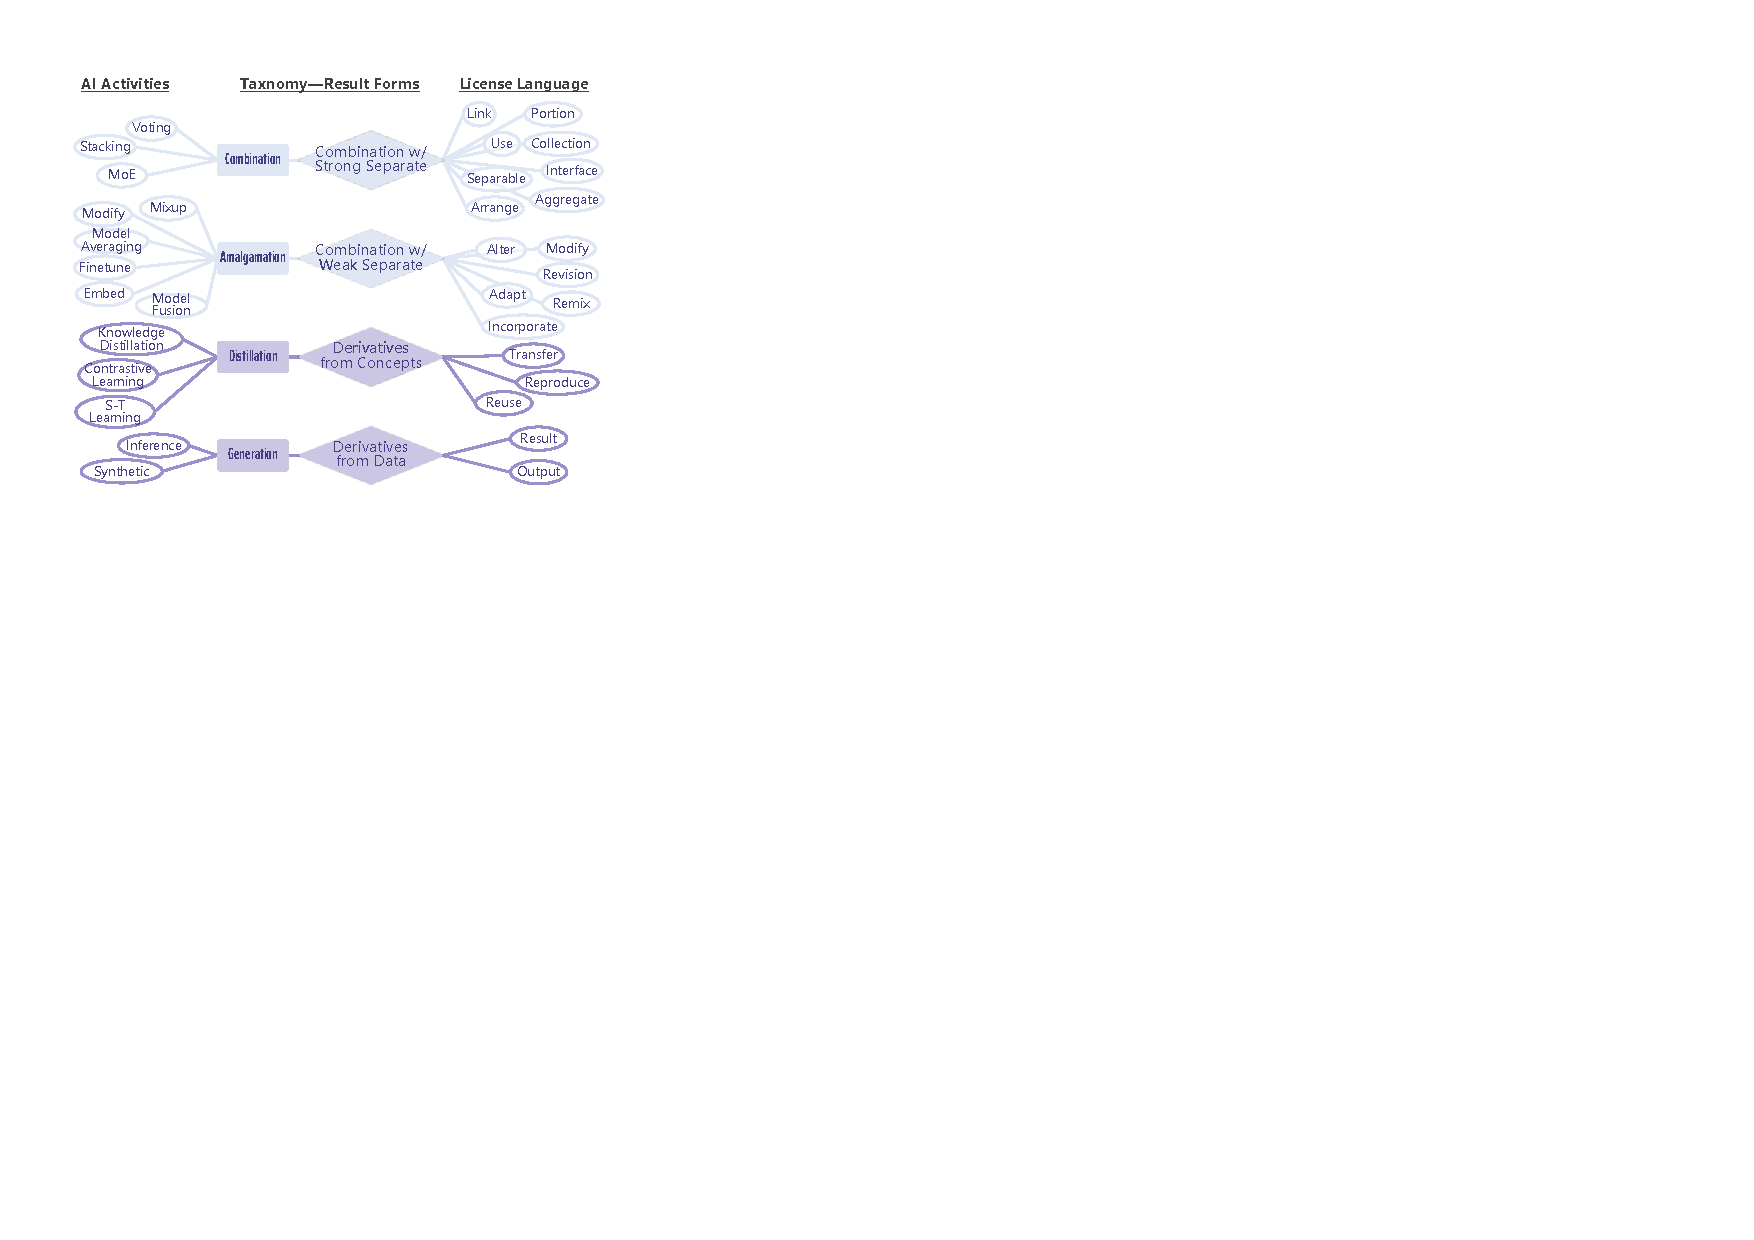
\includegraphics[width=\linewidth]{fig/taxonomy.pdf}
    \caption{Our proposed taxonomy bridging AI activities and license terms based on their result forms.}
    \Description{}
    \label{fig:tax}
\end{figure}

% 仅对于模糊定义而言,如果有明确定义那么优先级更高。 存在对应多种解释的情况,存在不同license的解释不通的情况  Train 的解释, 取决于对象
translated, altered, arranged, transformed, or otherwise modified 


Licensing Language Requires Standardization and  to ML and AI
the notion of derivative work is ill defined
conceptual ambiguities in existing licensing language
There is no consensus on whether the use

\begin{comment}
If CC SA-licensed content is included in a database, does the entire database have to be licensed under an SA license?

If CC SA-licensed content is included in a database, does the entire database have to be licensed under an SA license?
CC licenses never require a reuser of a CC-licensed work to make the original work or resulting works (collections, derivatives, etc.) publicly available. There are lots of private reuses of works that are permitted by CC’s licenses that do not require compliance with their terms. Regarding ShareAlike, the condition only applies if a work is modified and if the work is shared publicly. In the situation where a reuser created a dataset of photos and made it publicly available, and assuming copyright permission is required, then what is released is likely a collection or compilation of pre-existing works. CC licenses do not require the collection or the compilation itself to be made available under an SA license, even though each individual work is still licensed individually under an SA license and if they were modified by the distributor the modified photo would need to be licensed under the same terms. For example, were Creative Commons to compile photographs from a photo sharing website under a BY-SA 2.0 license and create a database that it then publicly distributed, CC could license the collection as a whole under a BY license, but the photographs would continue to be licensed under BY-SA 2.0.
\end{comment}